\chapter{TorTella Application}
In questo capitolo si parlerà del funzionamento dell'applicazione realizzata e di tutti i suoi meccanismi. L'argomento è incentrato su: bootstrap, flooding, failure detection, invio e ricezione pacchetti.
\section{BootStrap}
Il primo argomento riguarda il \textit{BootStrap} dell'applicazione, ovvero le operazioni effettuate per connettersi alla rete \textit{TorTella}. Per effettuare quanto detto si è deciso di fornire ad ogni peer una lista di coppie \textit{ip port} a cui connettersi inizialmente. Il metodo per reperire tale lista è al momento manuale (vedi \ref{conclusioni}). Le operazioni effettuate sono:
\begin{enumerate}
\item Viene avviata l'applicazione;
\item L'Applicazione prende un nodo dalla lista (ip e porta);
\item Avvia un \textit{client thread} che andrà a gestire l'invio di pacchetti verso il peer selezionato;
\item Il \textit{client thread} appena lanciato invierà inizialmente un pacchetto Ping (con fake recv\_ID), verso il peer a cui è associato, per stabilire la connessione;
\item Il peer ricevente risponde con un pacchetto di conferma e poi invia un Ping con il suo vero ID;
\item Il peer locale riceve il Ping e invia la conferma;
\item Connessione stabilita quindi torna al passo 2;
\end{enumerate}
Da questo elenco di azioni si può notare che avviene un invio del pacchetto Ping con fake recv\_ID, questo viene fatto perchè il peer locale che vuole entrare in TorTella Network non conosce l'ID dei nodi già presenti. Questo meccanismo di connessione che consente ai peer esterni alla rete di collegarsi senza problemi (vedi figura \ref{bootstrap}).
\begin{figure}[H]
\begin{center}
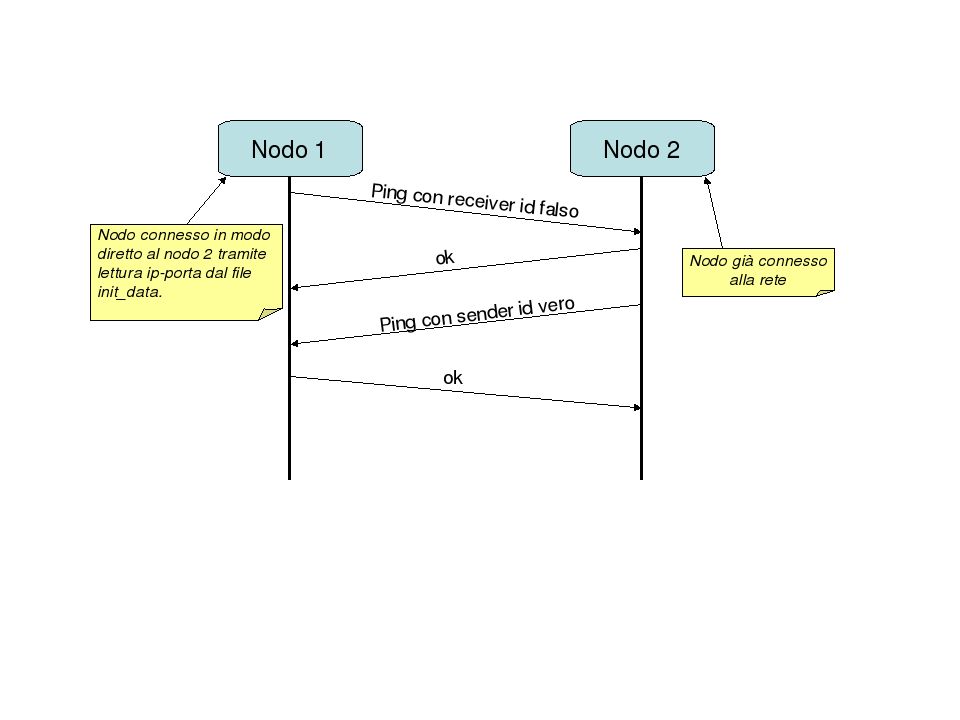
\includegraphics[scale=0.5]{etc/Bootstrap.png}
\caption{BootStrap peer}
\label{bootstrap}
\end{center}
\end{figure}
Il meccanismo di identificazione dell'ID di ogni nodo, connesso alla rete, si basa principalmente su un controllo con un parametro (\texttt{gen\_start}), opportunamente inizializzato nel file di configurazione. Seguendo l'esempio presentato in figura \ref{bootstrap}, il Nodo 1 dopo aver ricevuto il Ping dal Nodo 2 con il vero ID, esegue il controllo che il nuovo ID sia di valore maggiore rispetto a quello del parametro \texttt{gen\_start}\index{gen\_start}.
\section{Flooding}
Il meccanismo di \textit{flooding}\index{flooding} realizzato è stato ispirato a quello del protocollo \textit{Gnutella}, in cui quasi ogni pacchetto viene inviato in flooding. Nel caso di \textit{TorTella} vengono inviati in flooding i seguenti pacchetti: Search, SearchHits (\textit{backward routing}\footnote{segue a ritroso lo stesso cammino del rispettivo messaggio di Search}\index{backward routing}), Join e Leave. Essendo la rete in questione completamente decentralizzata, l'implementazione del flooding per gran parte dei pacchetti è stata una scelta dettata dal fatto che il protocollo \textit{TorTella} si basa fortemente sul \textit{passaparola}.
\subsection{Search e SearchHits}
L'intero meccanismo di searching delle chat, presenti nella rete, si basa sul principio del flooding, il quale provvede al re-direct di tutti i pacchetti di ricerca inviati da un generico peer, al fine di riuscire a recuperare una lista con tutte le chat attinenti alla query di ricerca.
Una forte limitazione che si potrebbe presentare, applicando tale algoritmo, consiste nella congestione dell'intera rete nel momento in cui il numero di peer connessi raggiunga quello di un'ipotetica \textit{web chat}\index{web chat}. Al fine di evitare il presentarsi di tale situazione è stato impostato ad un valore finito il campo \texttt{TTL}\index{TTL} (\textit{TIME TO LIVE}\index{TIME TO LIVE}) del relativo pacchetto di ricerca, il quale viene decrementato ogni volta che raggiunge un nodo, bloccando la possibilità di fare il redirect di un pacchetto nel caso questo abbia un valore pari a zero.
Di seguito viene riportato un esempio di possibile ricerca con tre nodi connessi.
\begin{figure}[H]
\begin{center}
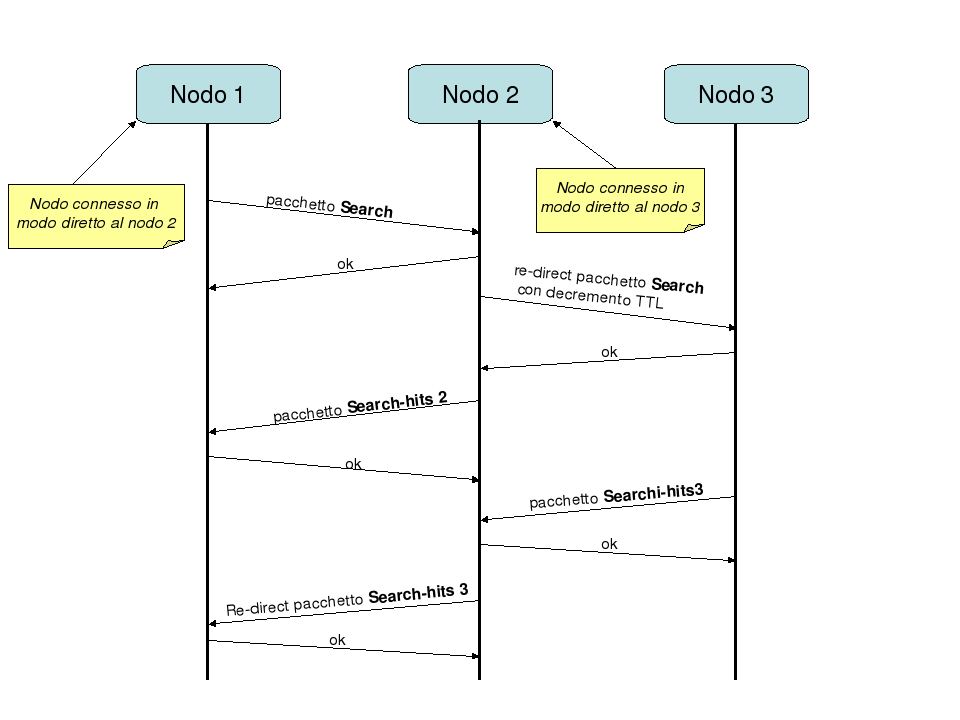
\includegraphics[scale=0.5]{etc/Search.png}
\caption{Search Flooding}
\label{searchflooding}
\end{center}
\end{figure}
Come è possibile notare osservando l'immagine \ref{searchflooding}, ogni nodo deve aver effettuato l'operazione di bootstrap per potersi connettere direttamente ai suoi  vicini. Successivamente il NODO 1 invia un pacchetto Search, che viene inoltrato agli altri nodi diminuendo di un'unità il valore del TTL. Il NODO 2 inoltra a sua volta il pacchetto e provvede a fornire la lista di tutte le chat da lui conosciute in quell'istante (inviando un SearchHits), che rispondano ai requisiti della query effettuata; infine il NODO 3 invierà la sua SearchHits al NODO 2 e quest'ultimo rinvierà tale pacchetto al NODO 1.
Il SearchHits sfrutta il \textit{backward routing}\index{backward routing} che consente ai peer di sapere a quali nodi rinviare il pacchetto quando ne ricevono uno. A tal proposito è stata realizzata una tabella di routing che contiene tutte le regole che ogni pacchetto con uno specifico ID deve seguire.
Un esempio di \textit{routing}\index{routing} può essere il seguente:
\begin{enumerate}
\item Un peer generico riceve un pacchetto Search;
\item Rinvia il Search ai suoi vicini e aggiunge una regola di routing per ognuno di essi;
\item Ogni volta che riceverà un SearchHits prenderà la regola di routing che il pacchetto deve seguire, ovvero il peer a cui deve essere rinviato.
\item Ogni regola ha un contatore, il quale viene incrementato in base a quanti pacchetti Search con uno specifico ID sono stati rinviati.
\end{enumerate}
\begin{figure}[H]
\begin{center}
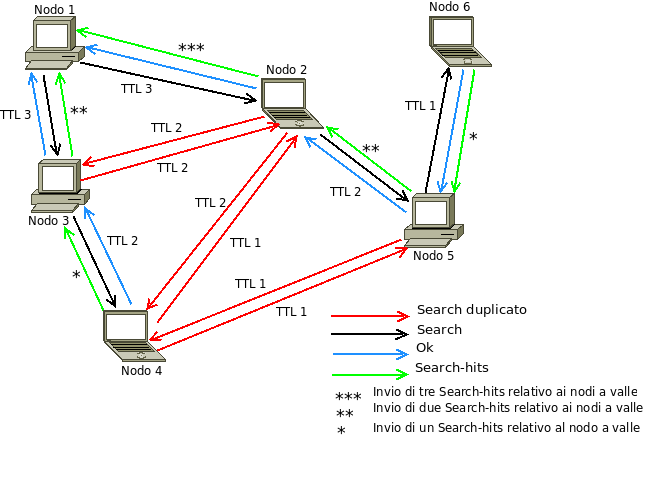
\includegraphics[scale=0.5]{etc/Search_overlay.png}
\caption{Search Flooding}
\label{searchoverlay}
\end{center}
\end{figure}
L'immagine in figura \ref{searchoverlay} ha lo scopo di evidenziare che il flooding dei pacchetti prevede un meccanismo di gestione dei pacchetti duplicati, ovvero ogni pacchetto di tipo Search possiede un identificativo univoco per tutta le rete, in questo modo se un peer riceve nuovamente un Search con lo stesso ID provvederà a scartarlo.
\subsection{Join}
Inviato nel momento in cui si tenta di accedere ad una chat, il pacchetto di Join segue un percorso di flooding di "sola andata", in modo che tutti i peer connessi alla chat a cui si sta accedendo aggiornino le proprie informazioni sui peer connessi. Inizialmente l'invio non doveva essere di flooding, ma in seguito a delle inconsistenze riscontrate nel caso di accessi simultanei alle chat, si è deciso di adoperare questa nuova politica. All'interno di un pacchetto di Join sono racchiuse tutte le informazioni riguardanti il peer che si sta' connettendo alla chat (che chiameremo peerA), poichè potrebbe accadere che alcuni peer raggiunti da tale pacchetto non conoscano il peerA. In questo modo, tutti i peer raggiunti saranno a conoscenza del fatto che peerA si sta connettendo ad una chat specifica e, nel caso uno di questi peer dovesse ricevere una Search, questi includerà nella lista degli utenti connessi (SearchHits) anche il peerA.
\begin{figure}[H]
\begin{center}
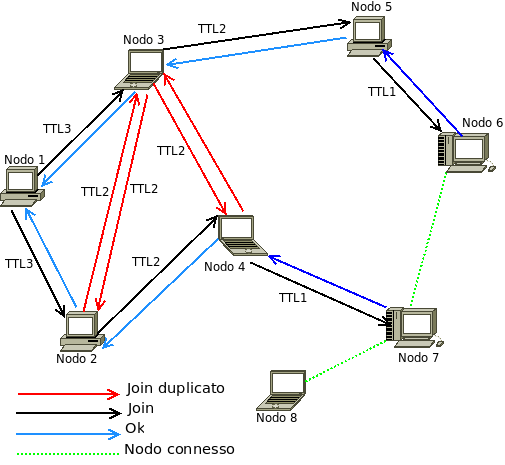
\includegraphics[scale=0.5]{etc/Join.png}
\caption{Join Flooding}
\label{joinflooding}
\end{center}
\end{figure}
\subsection{Leave}
Come il pacchetto Join, anche il Leave non era stato pensato come un pacchetto di flooding, ma viste le problematiche già incontrate con il Join si è adoperata la politica di flooding. Grazie al flooding, è stato possibile evitare problemi quali la presenza nella rete di differenti informazioni riguardanti le chat e i peer. Un tipico problema incontrato era il seguente: un peerA si sconnetteva dalla chat e inviava il Leave solo agli utenti connessi alla chat; questo comportava che qualora un qualsiasi peer effettuasse la ricerca di quella chat nell'istante in cui il peerA si stava sconnettendo, avrebbe ricevuto informazioni errate sulla chat, poichè il pacchetto SearchHits avrebbe contenuto tra gli utenti connessi anche il peerA.
\section{Failure Detection}
Tale meccanismo serve a capire quando un peer non è più attivo, a causa di crash o problemi di rete. Per la gestione di questi inconvenienti, si è deciso di inviare ad intervalli di tempo regolari un pacchetto di Ping per rilevare lo stato del peer remoto; in caso di mancato invio o errore nella ricezione del pacchetto, il sistema capisce che il peer remoto non è più attivo e provvederà alla rimozione dei dati che lo riguardano.
\begin{figure}[H]
\begin{center}
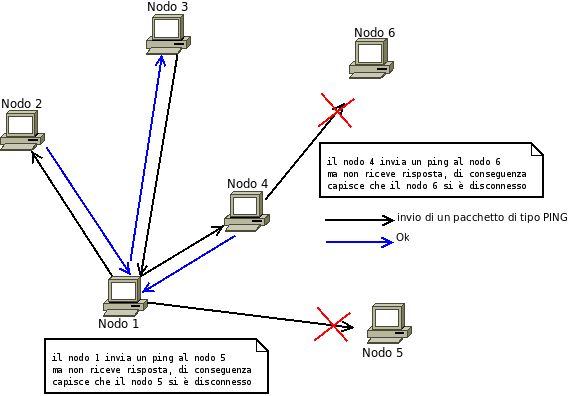
\includegraphics[scale=0.5]{etc/failure_detection.png}
\caption{Failure Detection}
\label{failuredetection}
\end{center}
\end{figure}
\section{Invio e ricezione dei pacchetti}
Per ogni peer con cui comunicare ci sono due thread: un thread per la gestione del client (invio) e un thread per la gestione del server (ricezione).
In questo modo se si vuole inviare un pacchetto ad uno specifico peer basta richiedere al \textit{client thread} di farlo, il che viene fatto sfruttando una semplice coda che contiene tutte le richieste di invio pacchetti. Il \textit{client thread} preleva la richiesta dalla coda ed effettua l'operazione desiderata.
Il \textit{server thread} invece riceve tutti pacchetti e li elabora in base al tipo (vedere capitolo \ref{architettura}). La comunicazione tra i thread ed il resto dell'applicazione è resa possibile da una struttura dati (una per peer) che contiene tutte le informazioni relative al peer. Tramite questa divisione dei compiti si è raggiunto un livello di efficienza tale da permettere la comunicazione con decine di peer contemporaneamente.
\section{Generazione ID}
Si sono scelti degli ID da 8 byte, in modo da rendere il più raro possibile la presenza di ID duplicati. Per la generazione dell'ID è stata usato un algoritmo che sfrutta il \textit{MAC}\index{MAX} della macchina e il \textit{timestamp}\index{timestamp}. Per dettagli vedere il capitolo \ref{architettura}.